\documentclass[format=acmtog, review=false]{acmart}

\begin{document}

\title{CS 265 Project: Log-Structured Merge Tree}
\author{Jack Dent}
\email{jdent@college.harvard.edu}
\maketitle

\section{abstract}
I present the design for a single-threaded Log-Structured Merge Tree (LSM Tree), as well as an implementation in C++. I show preliminary experimental results that suggest a buffer size of roughly 4MB optimises the throughput of the LSM Tree, and that increasing the buffer size does not yield additional benefits. Finally, I outline my design proposal for improving the write performance of the LSM Tree by splitting each level into a series of ``enclosures'', and the overall performance by leveraging parallelism.

\section{Basic Design}

The LSM Tree has two primary components: an in-memory buffer, and a number of on-disk data stores (``levels" or ``disk levels") of progressively increasing size. The LSM Tree makes a number of optimisations for efficient reads (GET, RANGE, and STATS queries). By storing the data in each of the disk levels in sorted order, the tree can retrieve individual keys using efficient binary search. Additionally, each disk level uses a bloom filter for fast membership testing, which improves the performance of GET queries. The LSM Tree, while optimised for reads, also aims to support efficient writes by buffering incoming key/value pairs in memory before flushing them to disk in larger batches. Flushing the buffer to disk - even amortized over multiple writes (PUT queries) - is an expensive operation which involves shuffling data across multiple disk levels, and I present a number of optimisations aimed to reduce its cost.

\subsection{GET queries}

The levels in the LSM Tree are ordered according to the recency of their entries. The buffer contains the most recent set of key/value pairs, while lower levels potentially contain progressively older data. To search for a key in the LSM Tree, we first search the buffer, and then search each of the disk levels in order of their depth. Currently, my buffer is an append-only log and does not enforce much structure on its key/value pairs. To find a given key we therefore resort to linear search, which takes $O(b)$ time in the worst case, where $b$ is the user-supplied parameter which controls the size of the buffer.

If we did not discover the key in the buffer, it is then necessary to search the lower disk levels. Every disk level stores its key/value pairs in ascending order without duplicates, and so we implement binary search to find a key. The binary search for a given level reads in $O(\log(bf^l))$ pages, where $f$ is the tree fanout, $l$ is the level depth, and $bf^l$ is therefore the maximum number of key/value pairs in the level.

Each disk level also keeps track of its member set of keys through a bloom filter. Whenever a key is written into a disk level, we hash the key using three different functions and set the bit at each of the hashed positions in a bitmask to the value of 1. When searching a disk level, we can immediately conclude that it does not contain the specified key if any one of the three bits as the hashed positions of that key in the bitmask is 0. Since bloom filters allow false positives, we will sometimes perform an unnecessary binary search during GET queries on a given level. Importantly, however, bloom filters never return false negatives, and so we will never fail to discover a key/value pair that actually resides within a disk level.

The size of the bloom filters is currently fixed at compile time and is equal across all levels. In the current state of the basic LSM Tree, it would be worthwile to explore two further optimisations:

\begin{enumerate}
  \item Tune the compile time parameter to find an appropriate value for expected workloads
  \item Allow the bloom filter size to vary between levels. Intuitively, levels whose size differ by an order of magnitude demand bloom filters of different size to optimise the space consumption to false positive rate.
\end{enumerate}

I take up these questions in the section on improving write performance.

\subsection{PUT queries}

The LSM Tree always inserts new key/value pairs into the buffer. If the buffer is full then the store will flush the buffer to disk before attempting to insert the key. To flush the buffer to disk, the store uses the following MERGE-DOWN($i+1$) procedure, starting with $i=0$ (the buffer is level 0):

\begin{enumerate}
  \item If level $i+1$ does not have space for the entries in level $i$, recursively call MERGE-DOWN($i+1$)
  \item Merge the entries in level $i$ with the entries in level $i+1$
  \item Empty level $i$
\end{enumerate}

After calling MERGE-DOWN($i+1$), we are guaranteed that level $i+1$ will be empty, which then allows us to merge level $i$ downwards. The final stage of the procedure clears level $i$ of entries, since they will now be contained by level $i+1$.

To merge two levels, we use an N-way external merge/sort procedure. We push the first entry in each of the levels, as well as the file pointer associated with that disk level, onto a priority queue which contains a list of (entry, file) pairs ordered by the entry key. While the priority queue is not empty, we pop the first tuple, writing the entry to a new file if the key is unseen, and discarding the entry if it contains the same key as the last one. If the file still has entries remaining, we read in the next entry and push the new (entry, file) tuple back onto the priority queue.

\subsection{DELETE queries}

DELETE queries are handled almost identically to PUT queries. To delete a key, the LSM Tree inserts the key with a tombstone value. By restricting the range of possible values to $[-2147483647, 2147483647]$, it is possible to assign $-2147483648$, the minimum value of a 32 bit integer, as the tombstone. Alternatively, if we did not want to restrict the value range, we could instead increase the size of the entries stored by the tree by an additional byte, which would indicate whether the deletion status of the associated key.

We keep tombstone entries until they reach the final level. When an entry reaches the final level, it is guaranteed that there are no deeper levels containing outdated values for that key. This observation allows us to remove tombstone entries from the final level, which prevents the tree becoming saturated with deleted key/value pairings.

\subsection{RANGE queries}

I use the N-way external merge/sort procedure outlined in the PUT query to serialize every key/value pairing in the store. This is hopelessly inefficient for most small RANGE queries, and I present a plan for improving its performance in the section on parallelisation.

\subsection{LOAD queries}

LOAD queries stream a binary file of key/value pairs, inserting each into the store in the sequence they occur. Thus, LOAD queries can be thought of as identical to a series of independent PUT queries, with the exception that they parse binary rather than ASCII data.

\section{Experimental results}

\begin{figure}
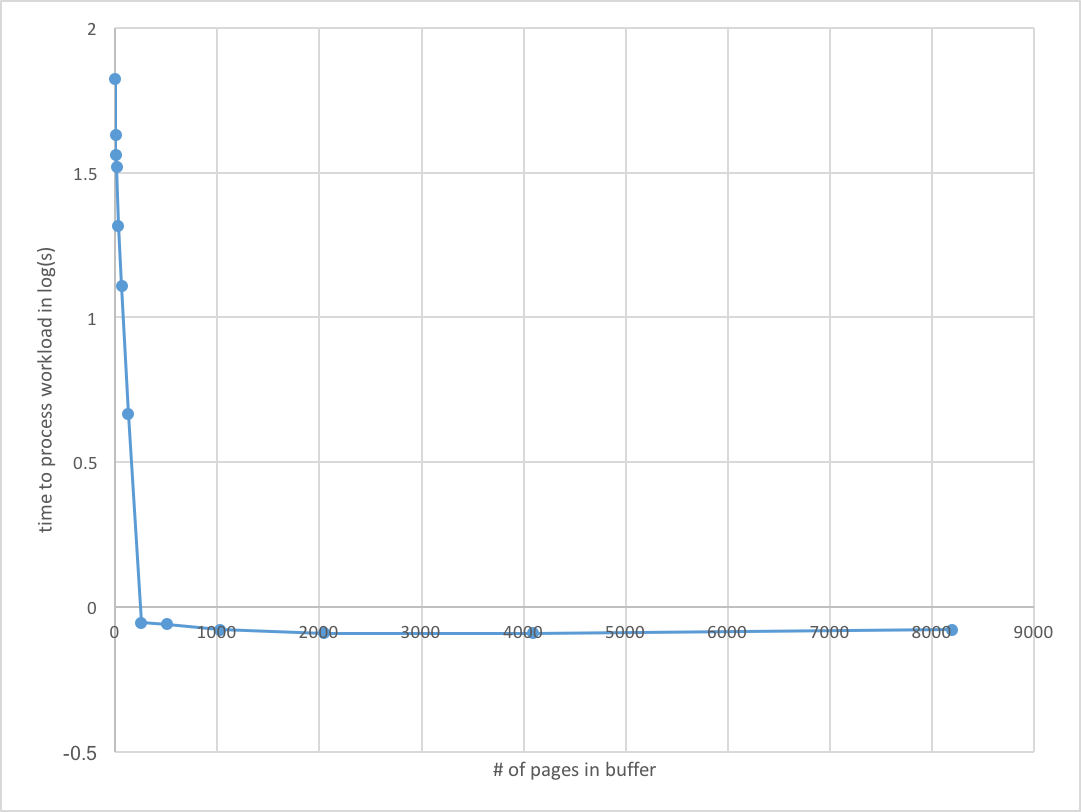
\includegraphics[width=3.3in]{chart}
\caption{Workload latency by buffer size}
\end{figure}

Figure 1 depicts how the performance characteristics of a number of different workloads vary according to the buffer size. I tested a number of different workloads with various distrubutions for each page size, and then averaged the time taken to complete the workload. The time axis is logarithmic.

\section{Future work}

\subsection{Improving write performance}

The cascading merge routine for the basic LSM Tree is very aggressive, which adversely impacts write performance. It requires a merge-sort every time the buffer becomes full, and also requires that entire levels are merged when upper levels become full. Merging two of the lower levels often takes a significant amount of time, during which all PUTs and GETs to the tree are blocked. By making the segmentation of the entries within each level more granular, we can reduce the complexity of the merge procedure and improve write throughput.

For the purposes of this paper, an ``enclosure" is a data structure containing a file pointer, a bloom filter, and fence pointers. Each disk level will store multiple enclosures, and for each enclosure we store the file pointer, bloom filter and fence pointers in memory. The file on disk contains key/value entries in sorted order, and at a maximum contains the number of entries in the buffer. Note that we can recreate the bloom filter and the fence pointers for an enclosure from the values on disk. The global ordering on the enclosures is given first by the ordering of the level to which they belong, and second by the time-ordering of the enclosures within that level, which gives them a pseudo-logical timestamp $i$. 

When merge/sorting $N$ enclosures, we create at most $N$ new enclosures with size bounded by the buffer size. This allows us to skip over more enclosures based on their fence pointers when performing GET/RANGE queries and thus perform less IO, which dominates the CPU-bound cost of fence-pointer filtering. It also allows us to fix the size of the bloom filter across all levels to an optimally tuned value, as well as model the complexity of queries more easily.

Rather than merging entire disk levels, the modified MERGE-DOWN procedure will flush a certain number of enclosures to the lower level to improve write performance. I plan to vary the policy that controls the number of enclosures to flush at each level in order to elicit varying read/write performance.

\subsection{Buffer data structure}

It is unlikely that the buffer will be the performance bottleneck for the LSM Tree, but I plan to implement a skip list to improve buffer reads and writes if I have time after implementing parallelisation.

\section{Parallelisation}

For the purposes of this paper, a ``threadpool" is a reusable pool of kernel threads. We use a threadpool for parallelisation so that we do not have to create a new set of threads for each query. The number of threads in the threadpool is denoted $t$, which should be tuned to optimal value for the hardware, which will often be the number of cores on the machine.

\subsection{GET queries}

Search the buffer. If no entry was found, then schedule the $t$ threads in the threadpool with monotonically increasing arguments in the range $[1, t]$. The argument reflects the enclosure id, effectively acting as a timestamp for the data the thread will search. The main thread waits for all threads in the threadpool to complete and then returns the value stored in a global variable shared across all the threads (which is initially set to nullptr).

To search an enclosure, the thread first checks the fence pointers to make sure the key is in range, and then reads the enclosure data from disk into main memory, performing a binary search to find the value. If the thread discovered a key/value pair, and if that key/value pair is more recent than the pair discovered by all other threads to that point, it sets the value and the enclosure id in shared memory. The thread then checks to see whether it should schedule itself again with the next lowest enclosure id, which happens if and only if three conditions hold:

\begin{enumerate} 
  \item The value stored in global memory is still nullptr; and
  \item there are remaining enclosures to search. 
\end{enumerate}

The threads use a spinlock to enforce mutual exclusion around the shared memory, which contains three variables: the lowest un-searched enclosure id, a pointer to the value variable, and a variable containing the id of the enclosure in which the value variable was discovered.

\subsection{PUT/DELETE queries}

When there are fewer than $c\cdot t$ enclosures to be merged, where $c$ is a variable parameter (initially set to $c=2$), I merge the entries in a single thread. Otherwise, each thread merges a subset of the encolsures, which are uniformly partitioned across the threads, and write their intermediate results to a temporary file on disk. When each of the threads have finished merging their enclosures, I perform a $t$-way external merge/sort on the temporary files and add the new enclosures to the appropriate disk levels.

\subsection{RANGE queries}

Stage 1 - filtering: the main thread creates an ordered queue of enclosures to merge/sort, where we push an enclosure onto the queue if and only if the target range overlaps with the enclosure's fence pointers.

Stage 2 - $t$ ($t/|Q|$)-way merge/sorts: We partition the queue into $t$ non-overlapping ordered subarrays, launch a threadpool, and assign the $i^{th}$ thread to merge/sort and filter the $i^{th}$ queue subarray into new main memory storage.

Stage 3 - $t$-way merge/sort: The main thread waits for all the threads in the threadpool to complete, and then performs a $t$ way merge/sort on the entries in the temporary main memory stores created by each thread.

\end{document}
